\newpage
\subsection{Figure Legends}\label{figure-legends}

\textbf{Figure 1.} Actual aerial strip transect tracks (gray lines)
during winter (October - April, 2003 - 2005) sea duck surveys (n = 30)
in Nantucket Sound, Massachusetts, US. The grid indicates the extent of
the 1100 km\textsuperscript{2} study area and its division into 504
2.25km\textsuperscript{2} segments. The polygon in northwest Nantucket
Sound indicates the 62 km\textsuperscript{2} area of permitted wind
energy development on Horseshoe Shoal.

\textbf{Figure 2.} Marginal functional plots for stably selected
covariates in the occupancy (probability of presence) and conditional
abundance (mean and overdispersion of count models) of Common Eider
(COEI), scoter (SCOT), and Long-tailed Duck (LTDU) in Nantucket Sound
during three winters, 2003 - 2005. Plots illustrate the partial
contribution to the additive predictor (Y-axis) of a covariate holding
all other covariates at their mean. Within a model, univariate plots
(i.e., lines) share a Y-axis scale, enabling direct comparisons of
effect sizes among covariates and species. For bivariate plots, the
Y-axis and X-axis reflect the first and second variables listed in the
interaction, respectively; colors indicate the direction and magnitude
of the partial contribution (blacks = negative, reds = positive; darker
colors = larger effect) and are likewise comparable within a model.
Northing by easting effects are given only at 31 December. For factor
variables, only the general association (i.e., positive or negative)
with the additive predictor is given. Covariate abbreviations correspond
to Equation 1.

\textbf{Figure 3.} Occupancy probability for Common Eider (COEI), scoter
(SCOT), and Long-tailed Duck (LTDU) in Nantucket Sound during three
winters, 2003 - 2005. Occupancy probabilities (top row) represent the
median expected probability of sea duck presence in a 1.5 km x ca. 180 m
transect through a given segment predicted on 10 evenly-spaced dates
from 15 November through 1 April in each winter. Spatiotemporal
variation in occupancy (\%; bottom row) is indicated by the median
absolute deviation, MAD, of occupancy probability relative to the
median. Predicted values are categorized based on their quartiles;
segments with the highest occupancy or variability (values \(\geq\) 98th
percentile) are outlined in black.

\textbf{Figure 4.} Conditional abundance of Common Eider (COEI), scoter
(SCOT), and Long-tailed Duck (LTDU) in Nantucket Sound during three
winters, 2003 - 2005. Conditional abundances (top row) represent the
median expected number of sea ducks, assuming their presence, in a 1.5
km x ca. 180 m transect in each segment predicted on 10 evenly-spaced
dates from 15 November through 1 April in each winter. Spatiotemporal
variation in conditional abundance (\%; bottom row) is indicated by the
median absolute deviation, MAD, relative to the median. Predicted values
are categorized based on their quartiles; segments with the highest
conditional abundance or variability (values \(\geq\) 98th percentile)
are outlined in black.

\textbf{Figure 5.} Unconditional abundance of Common Eider (COEI),
scoter (SCOT), and Long-tailed Duck (LTDU) in Nantucket Sound during
three winters, 2003 - 2005. Median abundances (top row) represent the
expected number of sea ducks along a 1.5 km x ca. 180 m transect within
each segment predicted on 10 evenly-spaced dates from 15 November
through 1 April in each winter. Spatiotemporal variation in abundance
(\%; bottom row) is estimated from the median absolute deviation, MAD,
relative to the median. Predicted values are categorized based on their
quartiles; segments with the highest abundance or variability (values
\(\geq\) 98th percentile) are outlined in black.

\textbf{Figure 6.} Relationship between observed and predicted total
abundance of Common Eider (COEI), scoter (SCOT), and Long-tailed Duck
(LTDU) during 30 aerial surveys of Nantucket Sound over three winters,
2003 - 2005. The dashed line indicates a 1:1 relationship between
predicted and observed abundances in surveyed segments; points below and
above this line indicate underestimates and overestimates of predicted
abundances, respectively.

\newpage

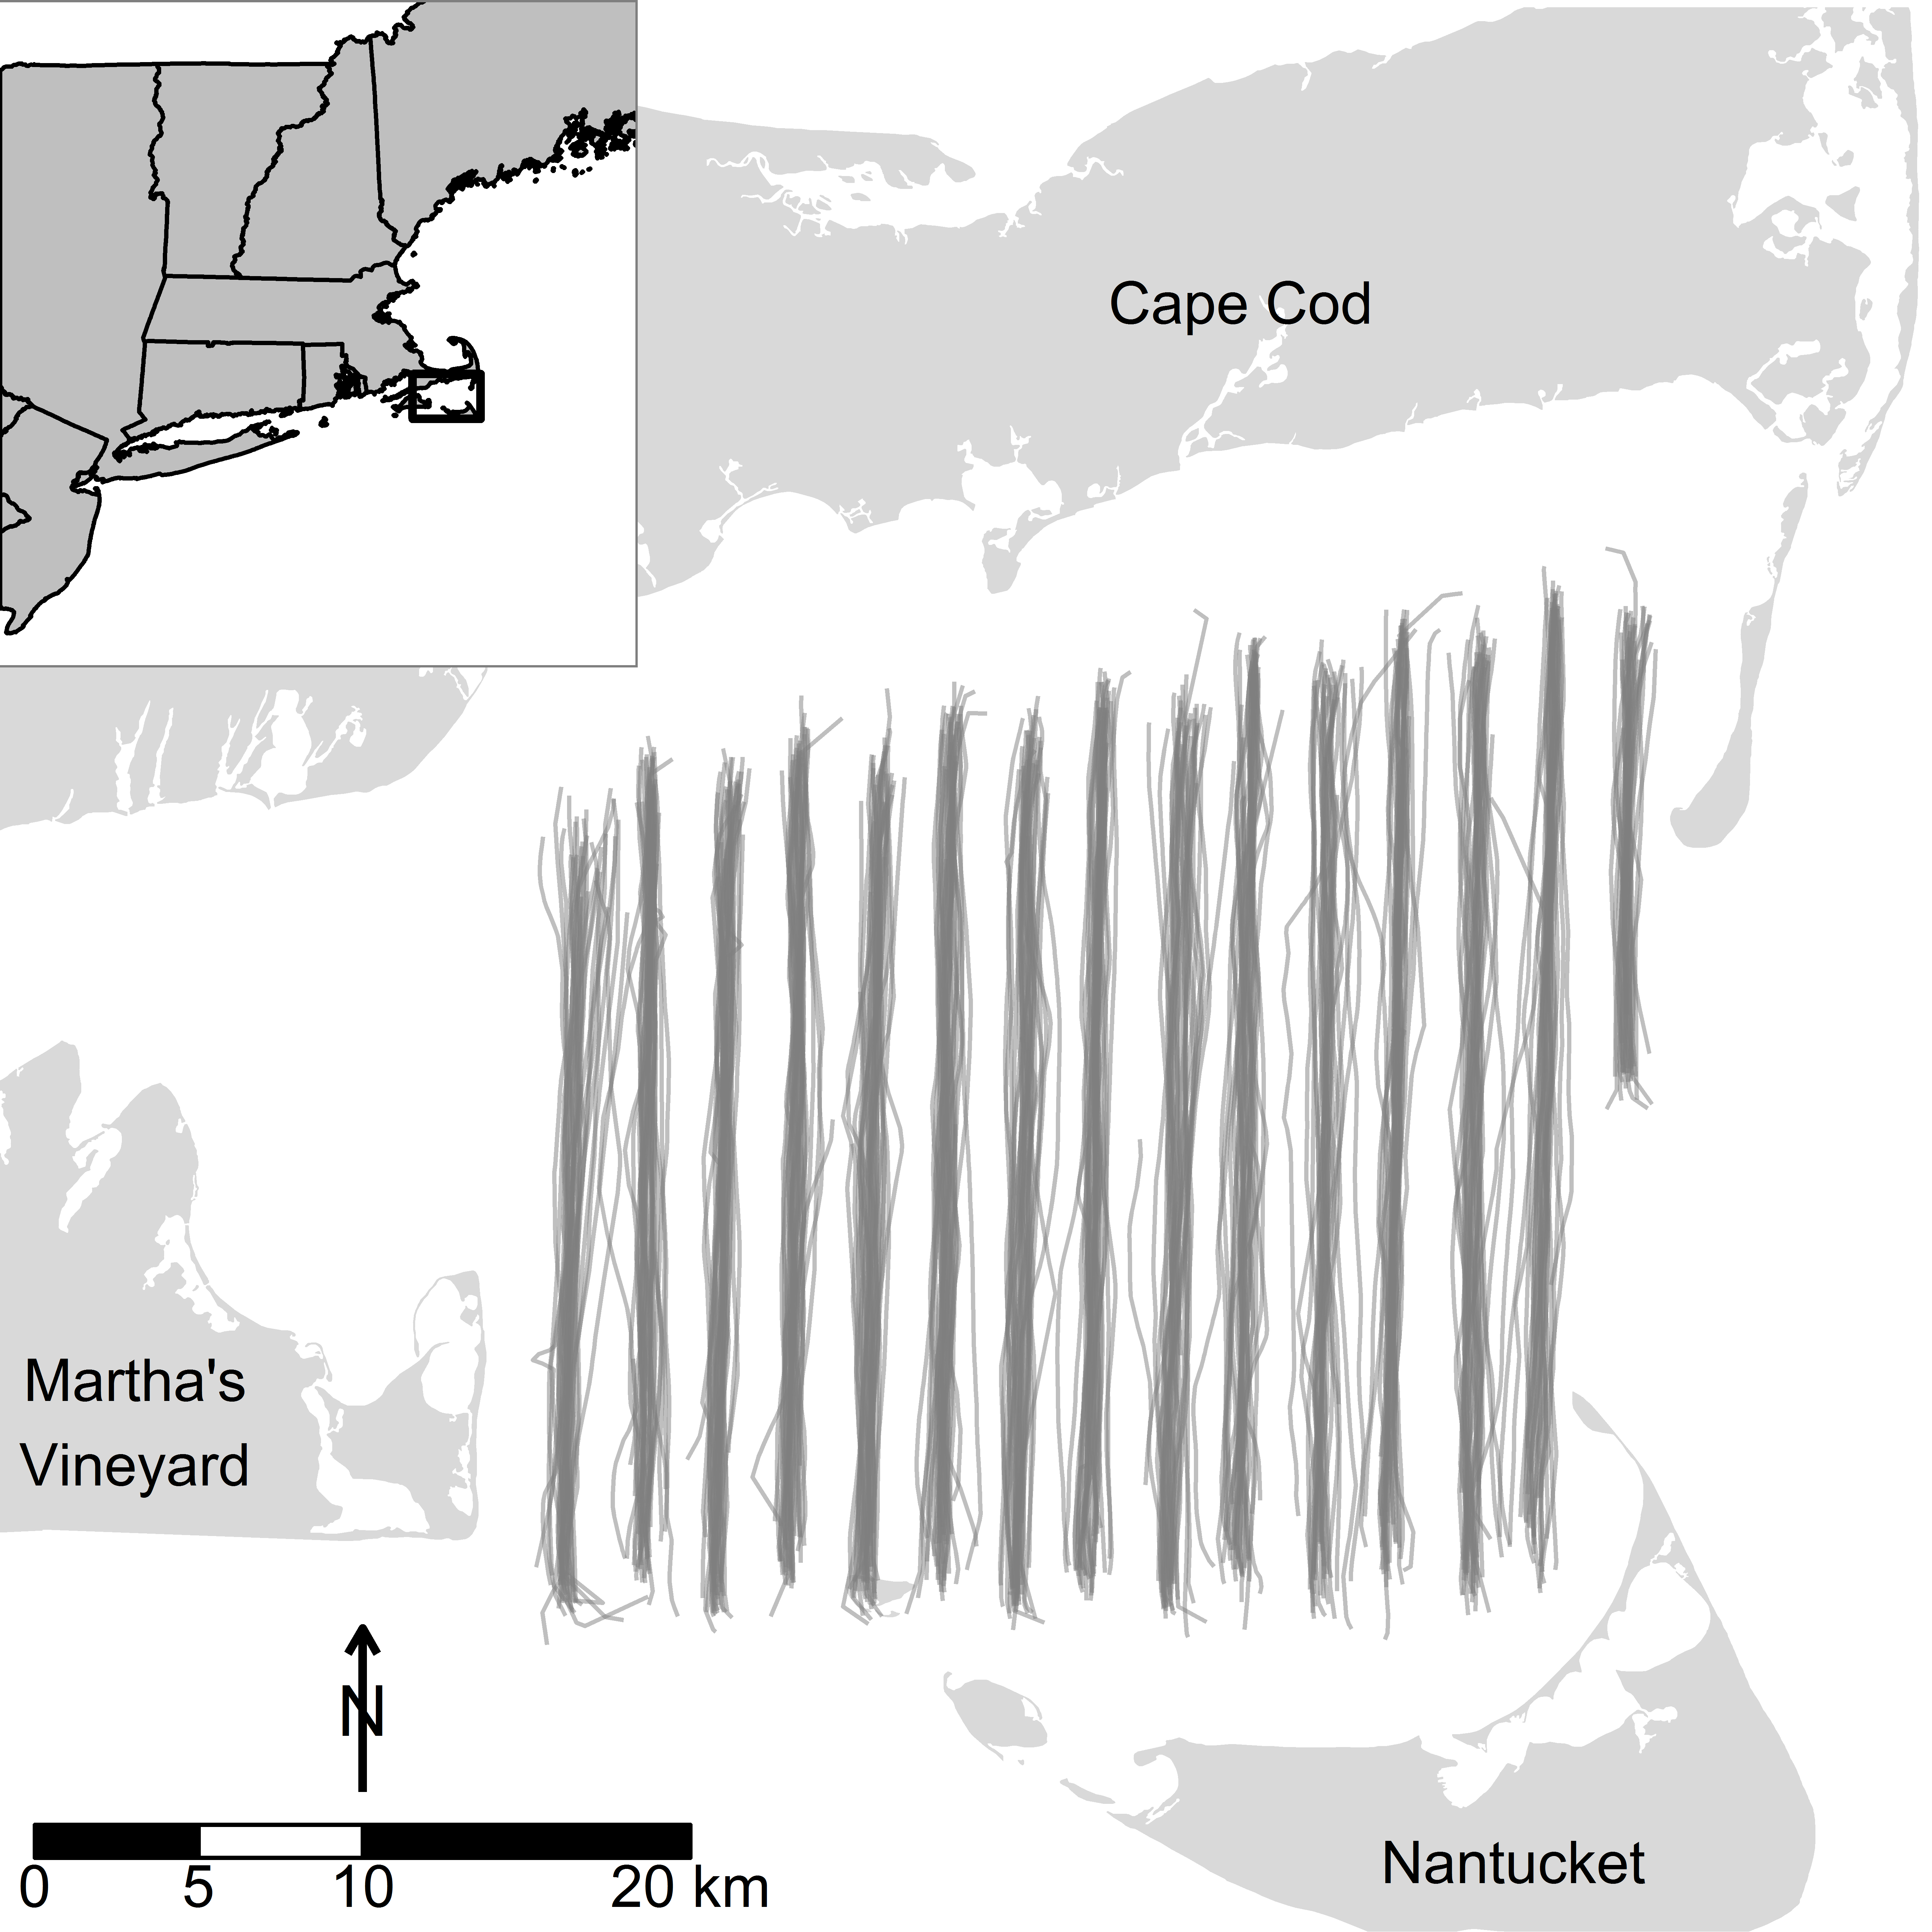
\includegraphics{./Figures/Nantucket_study_area.png}\\
\textbf{Figure 1}

\newpage

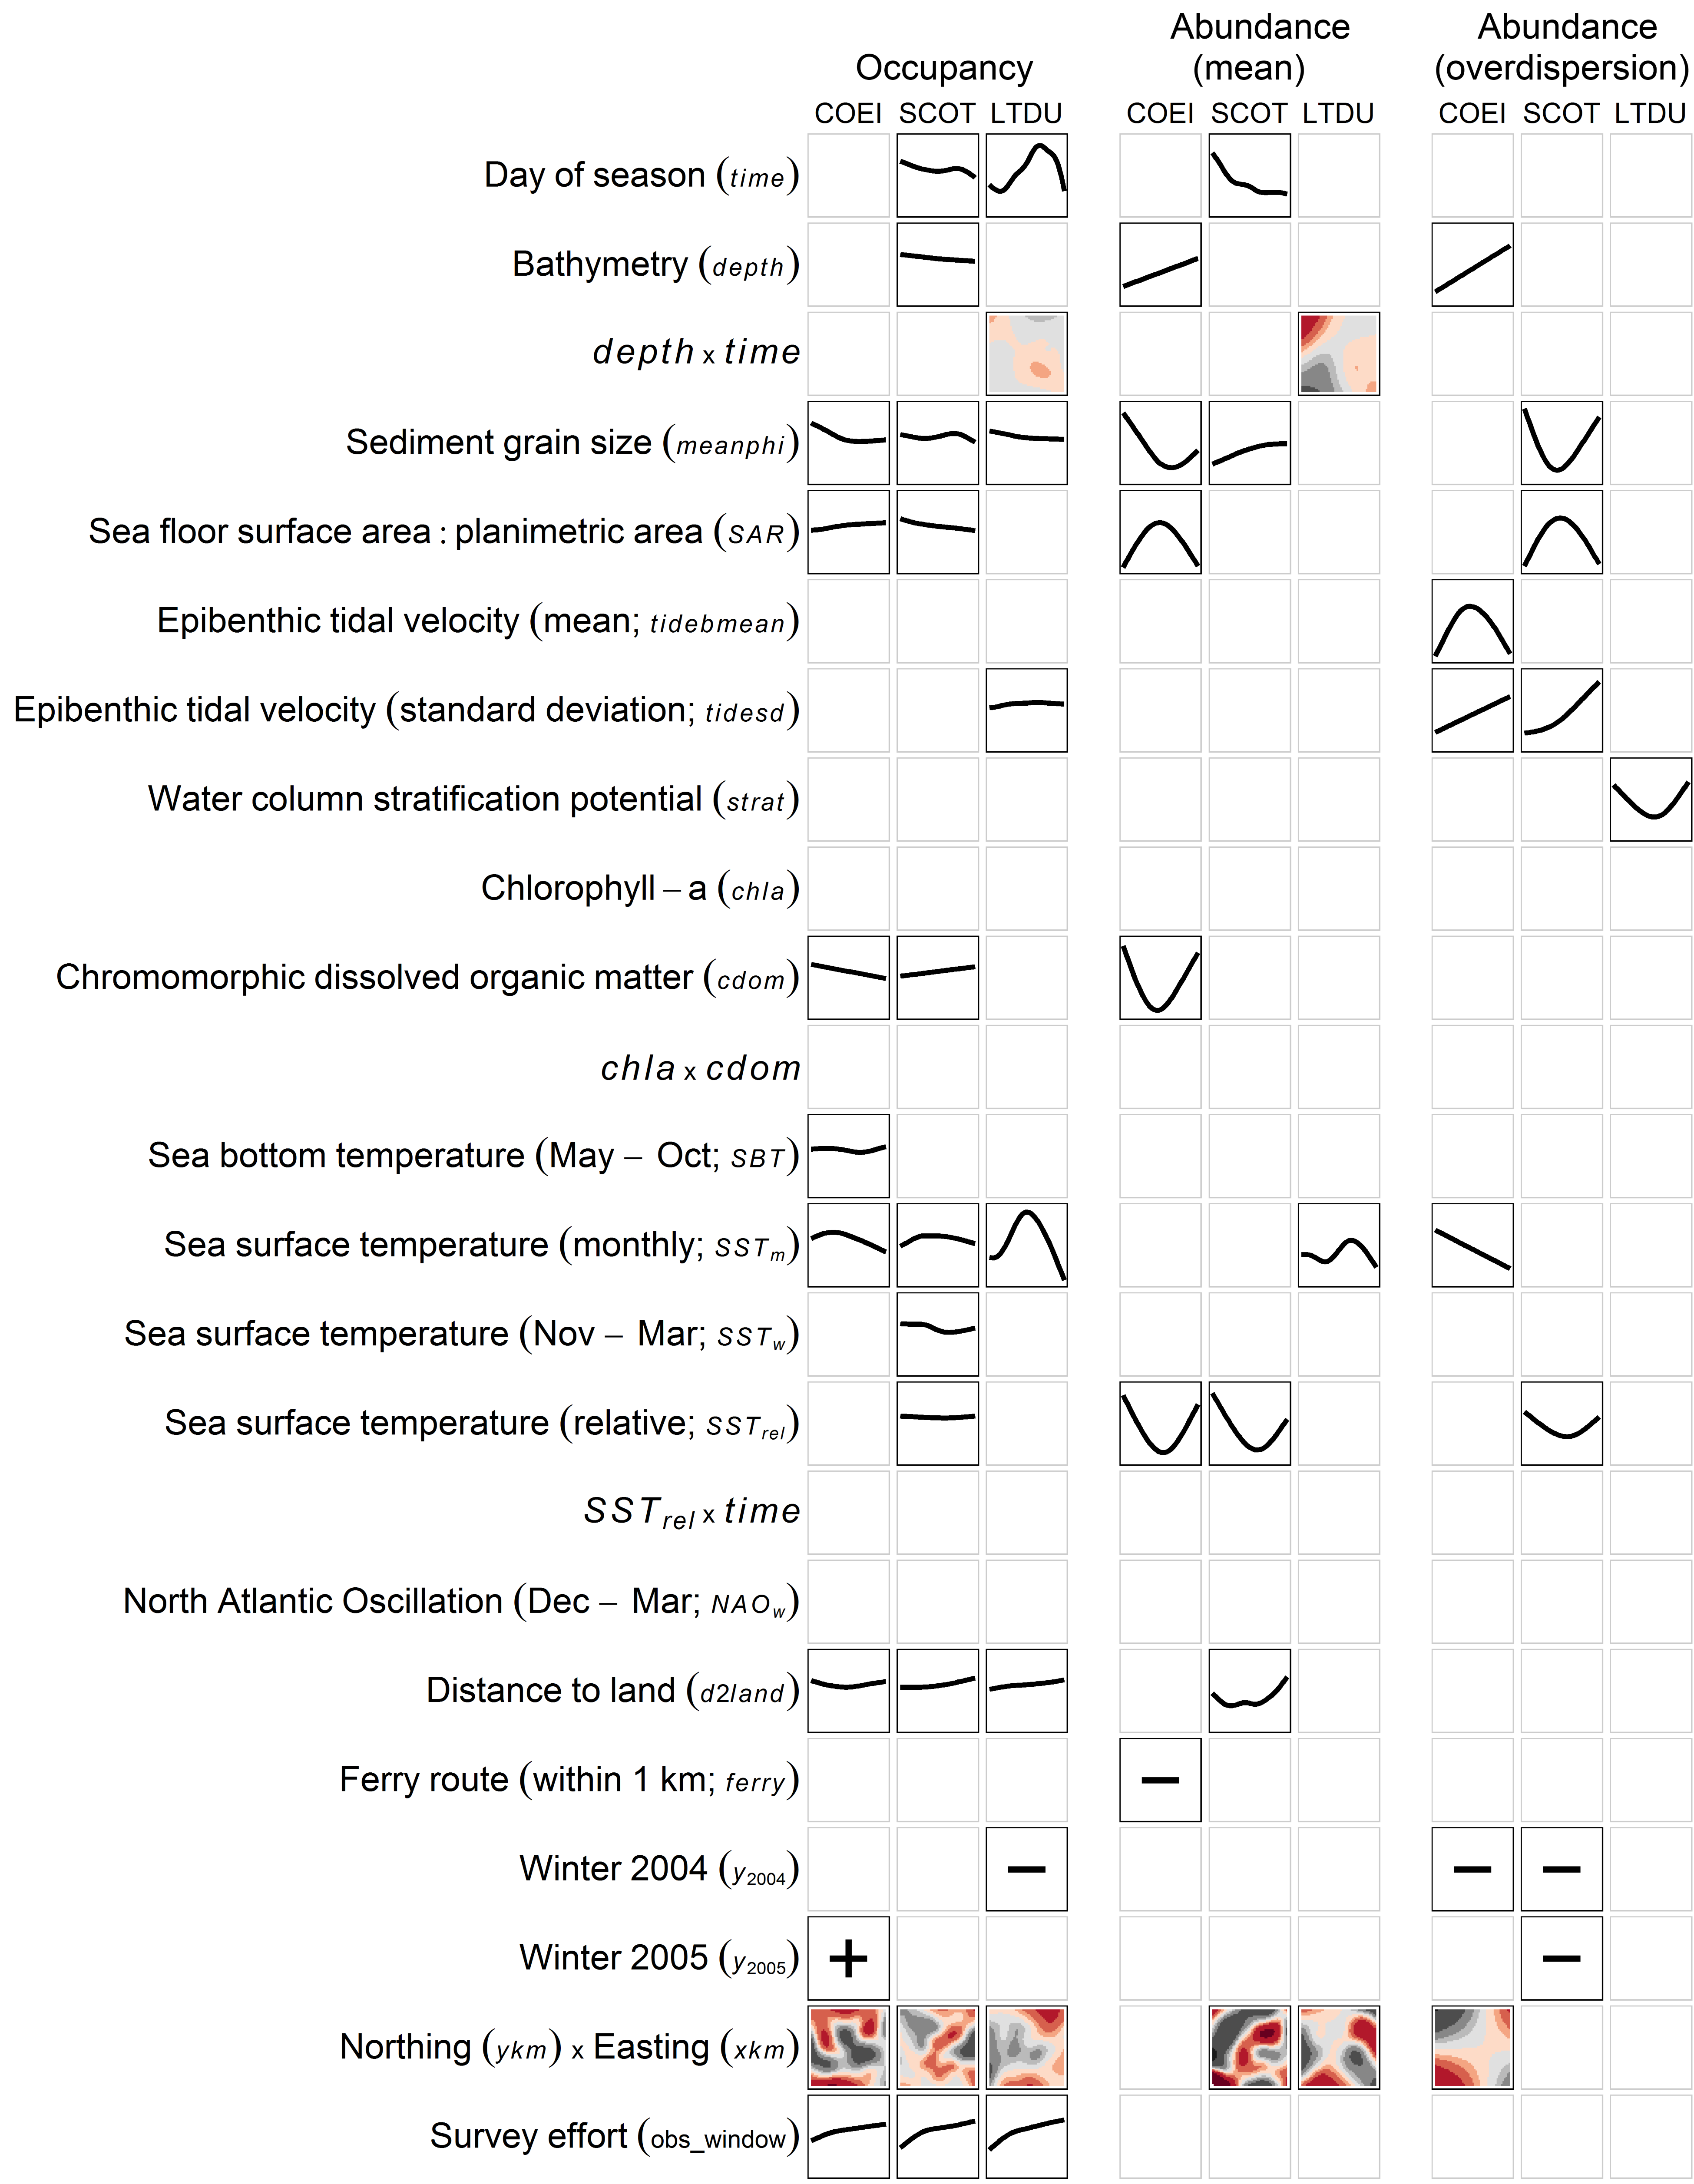
\includegraphics{./Figures/Covariate_effects.png}\\
\textbf{Figure 2}

\newpage

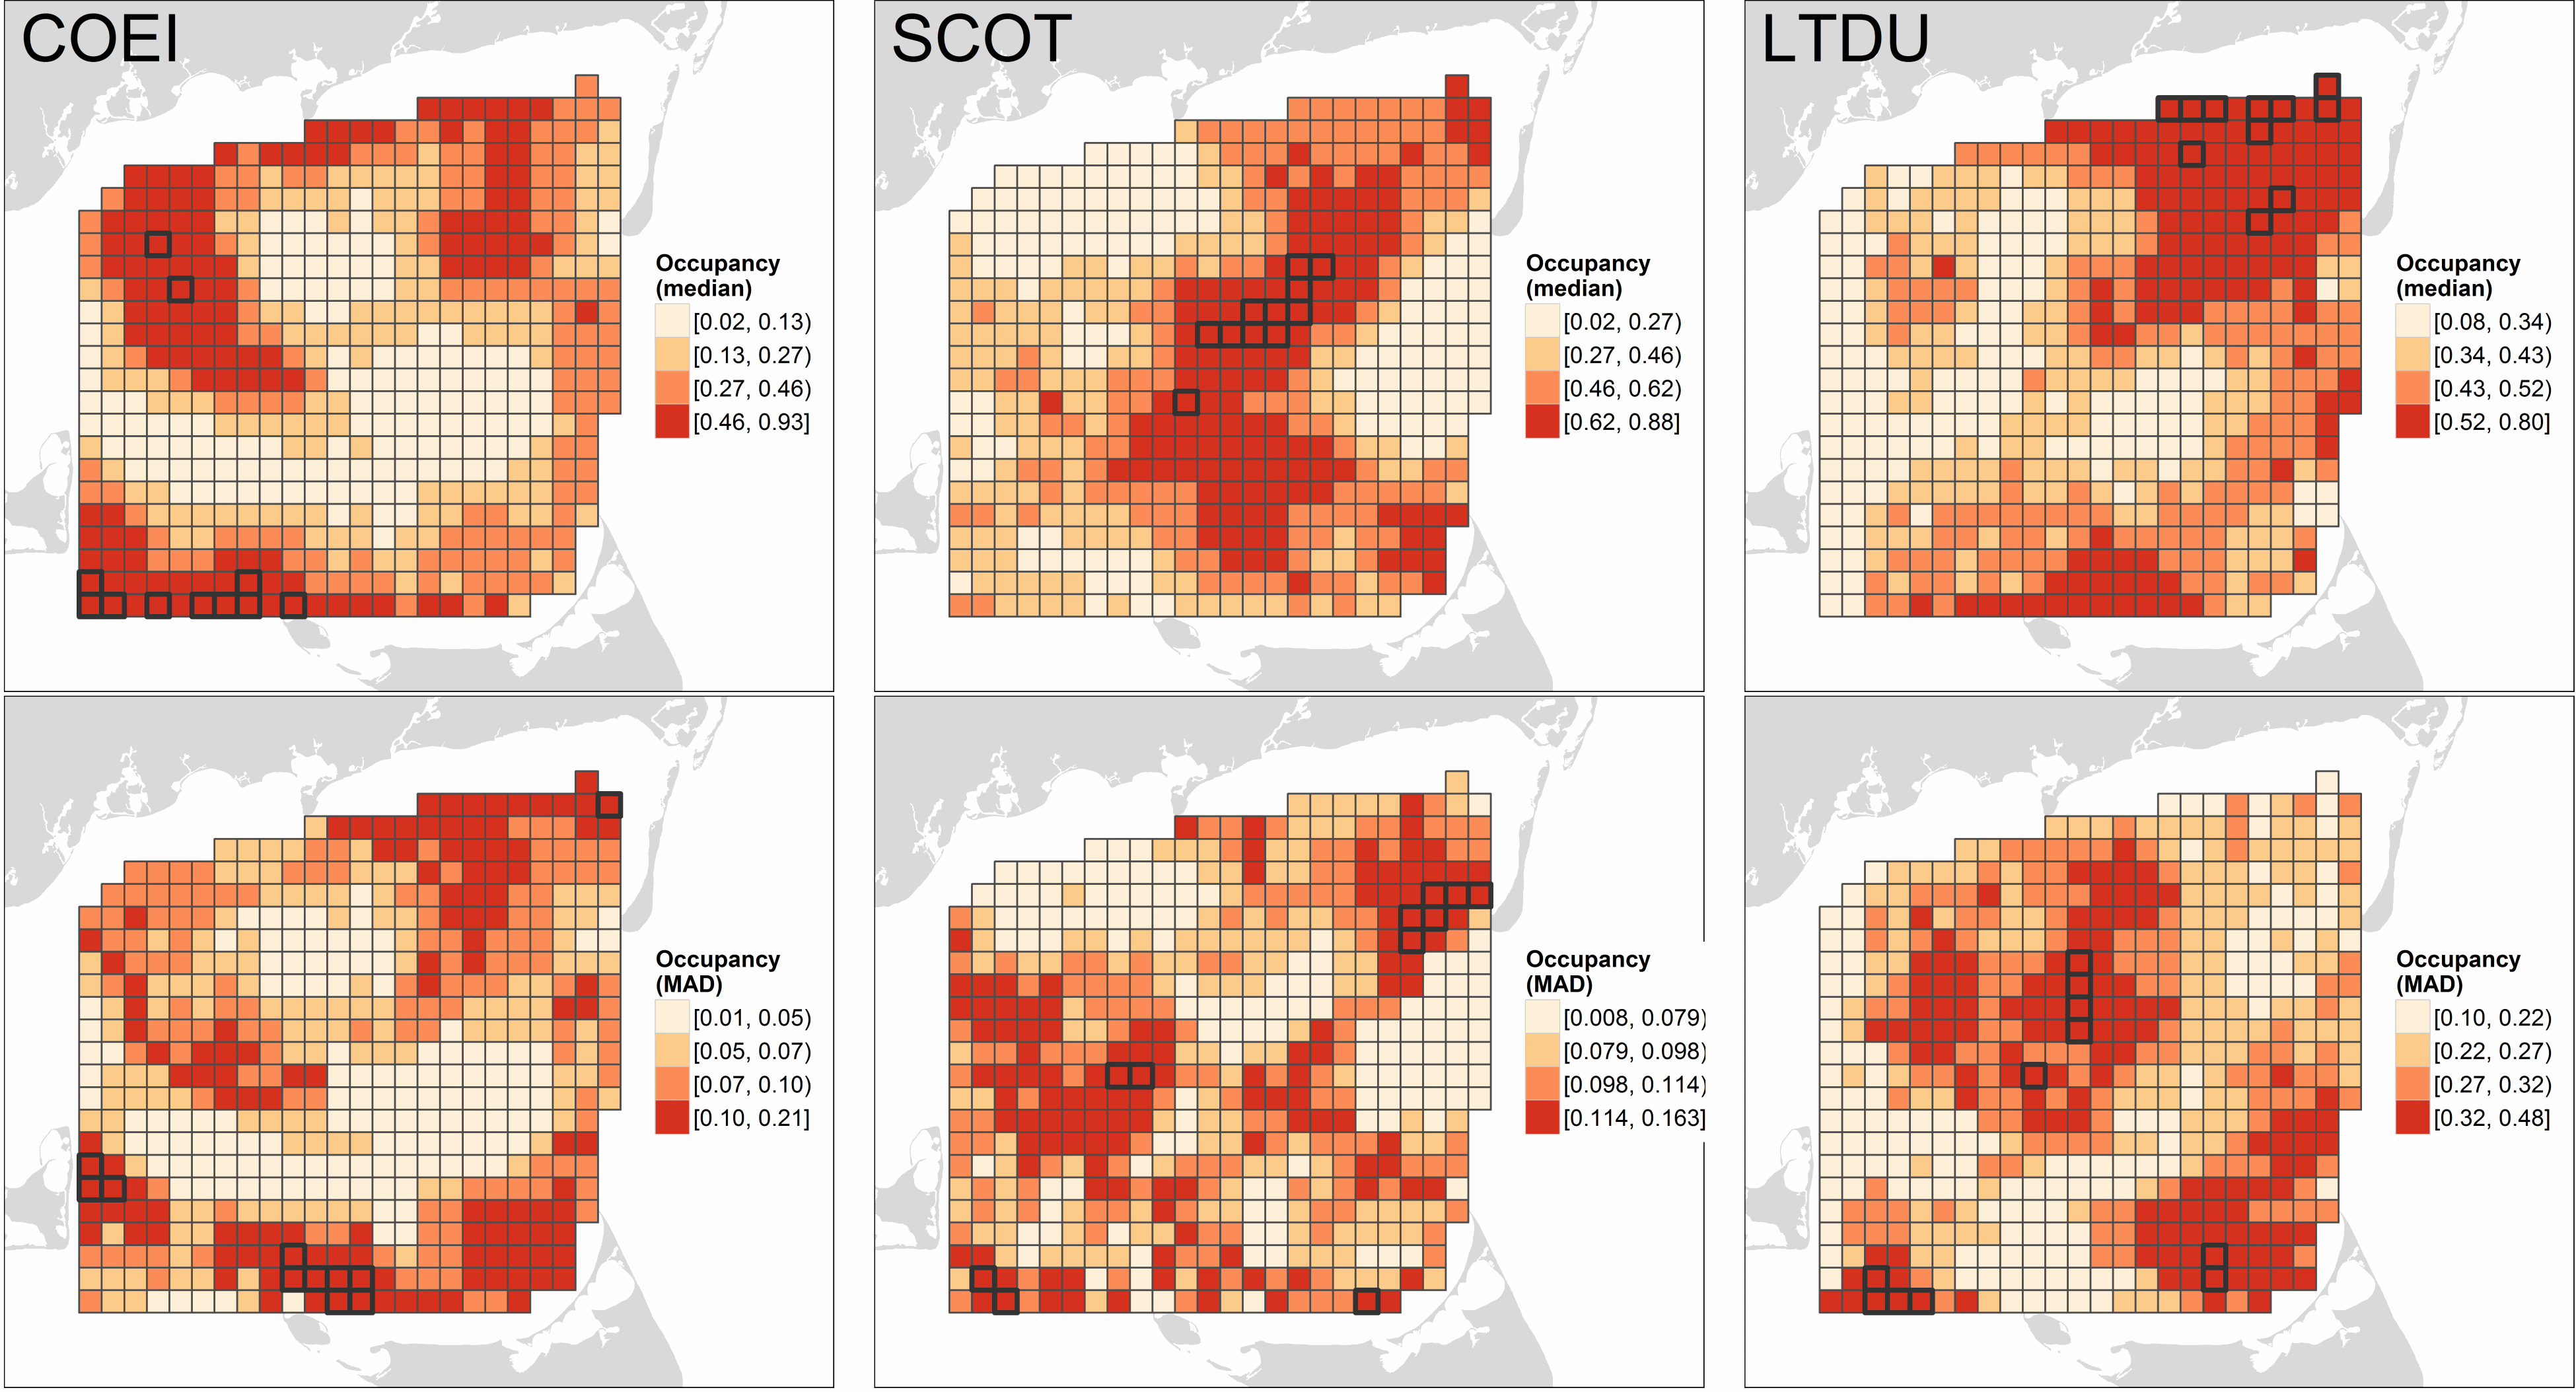
\includegraphics{./Figures/occupancy_maps_reduced.png}\\
\textbf{Figure 3}

\newpage

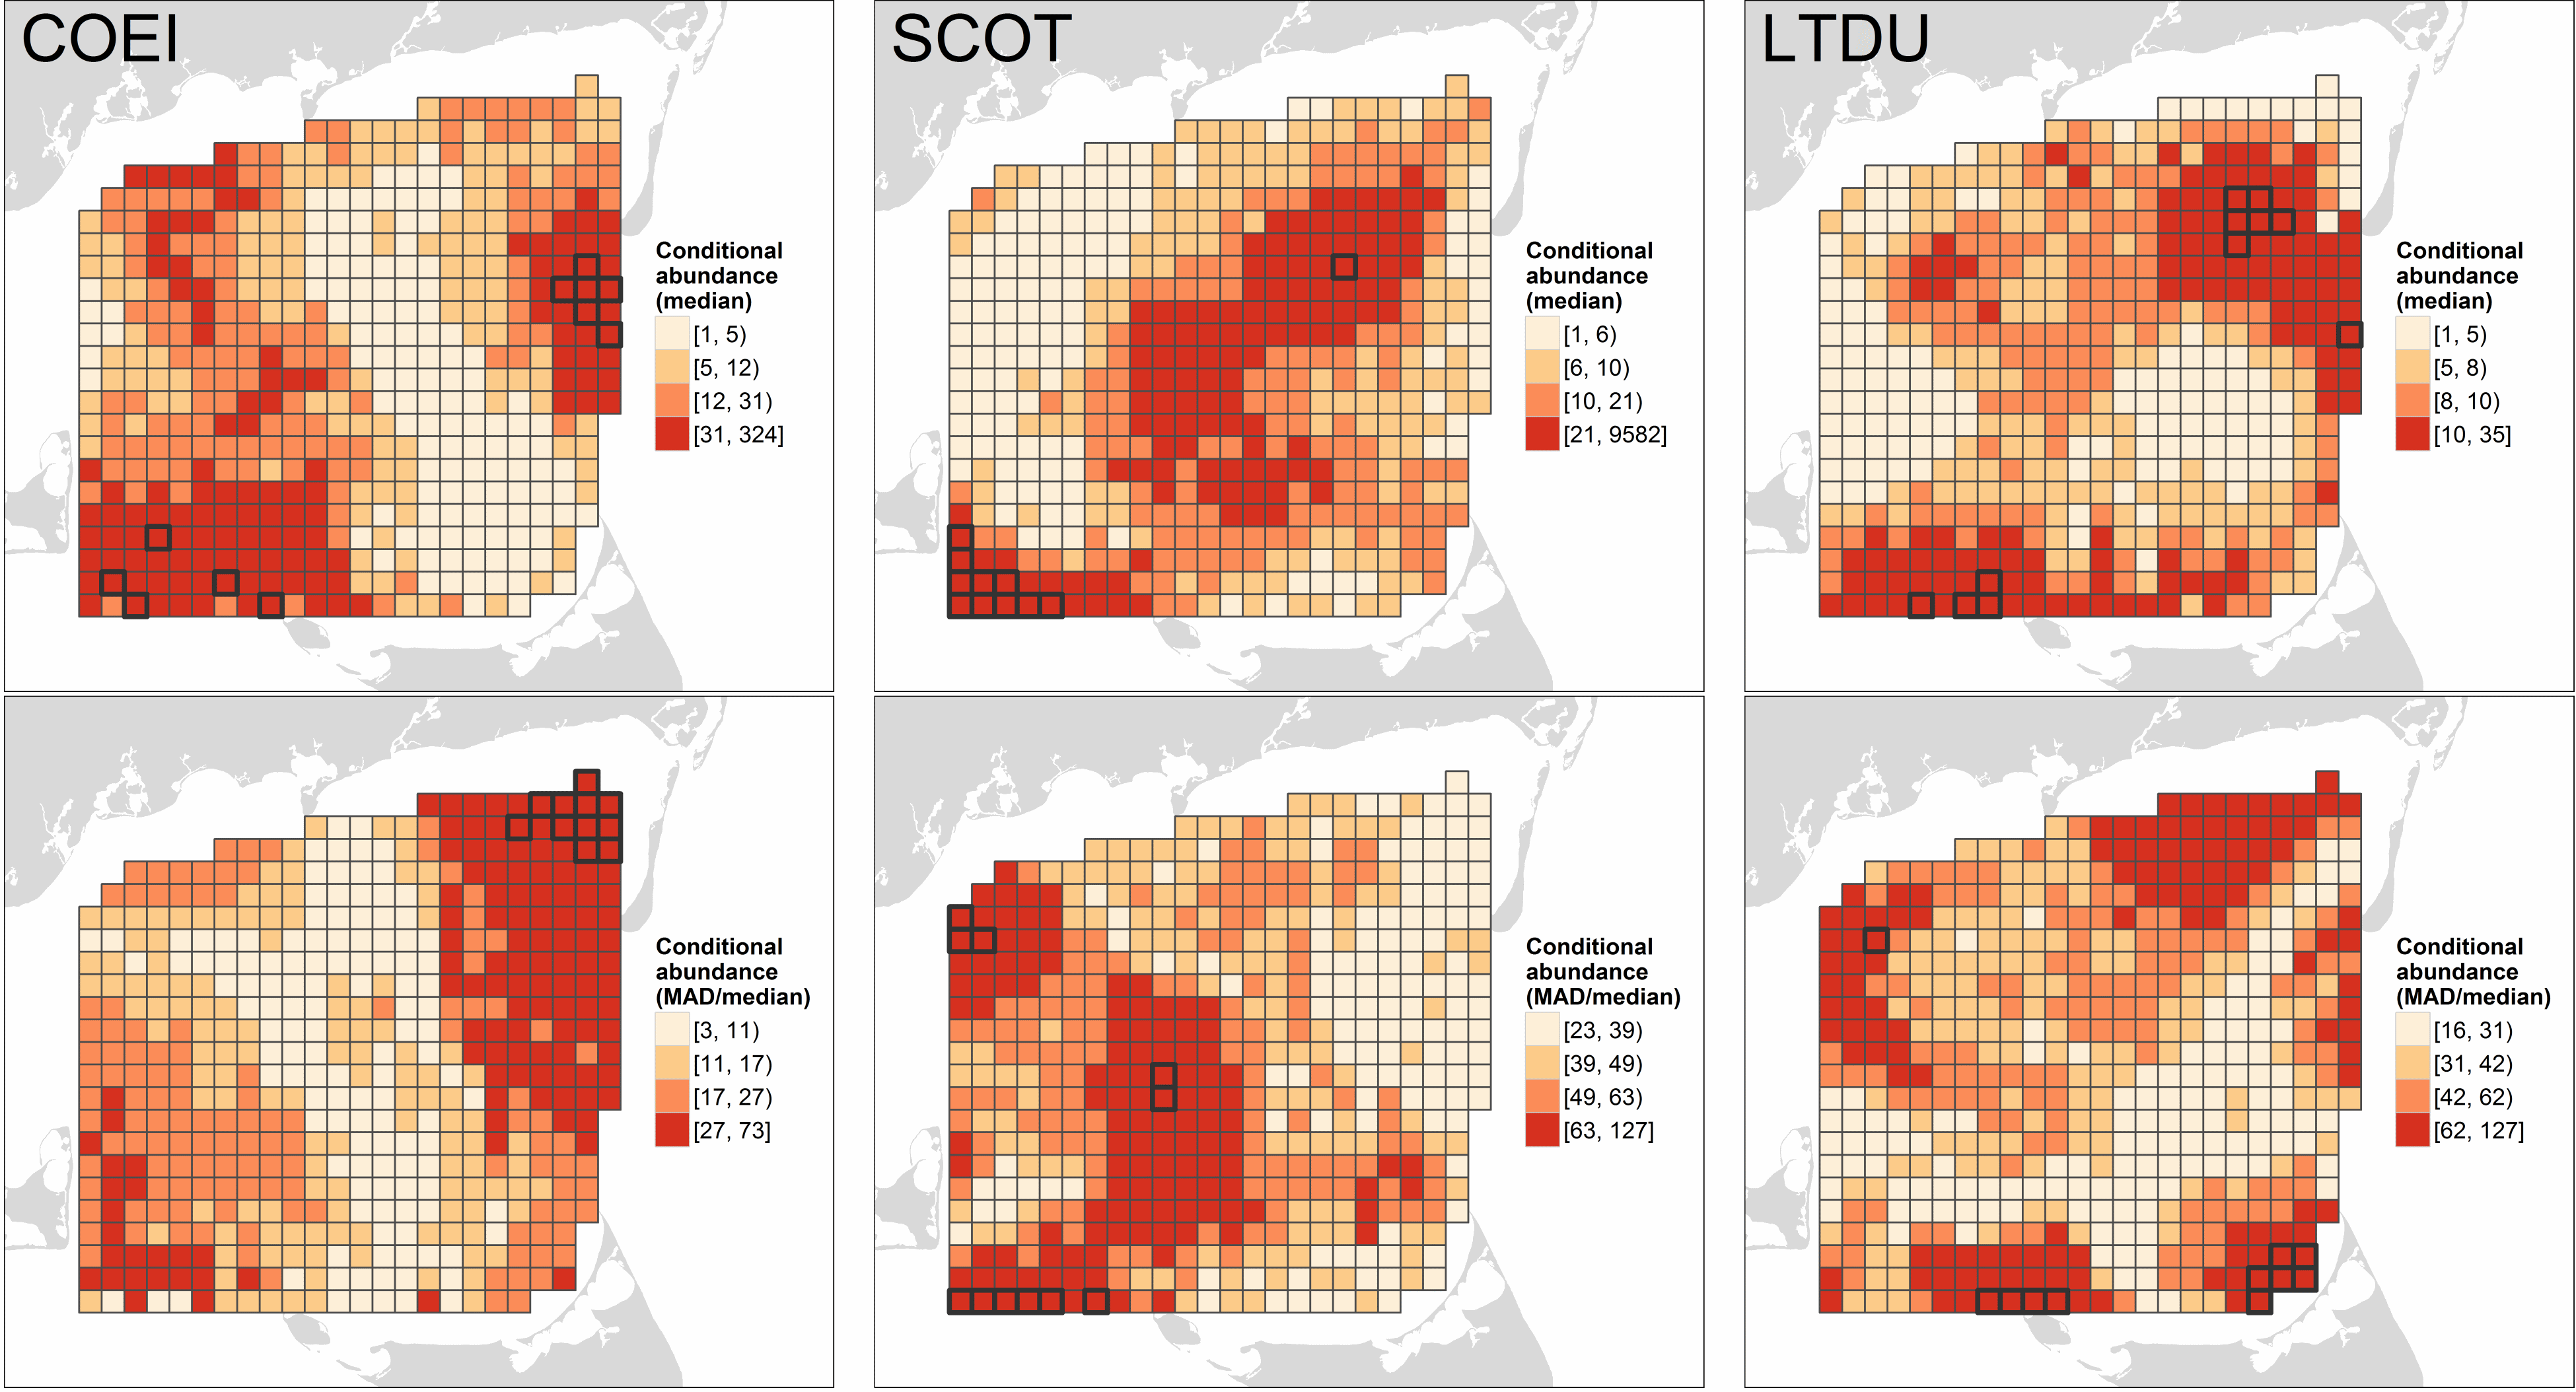
\includegraphics{./Figures/conditional_abundance_maps_reduced.png}\\
\textbf{Figure 4}

\newpage

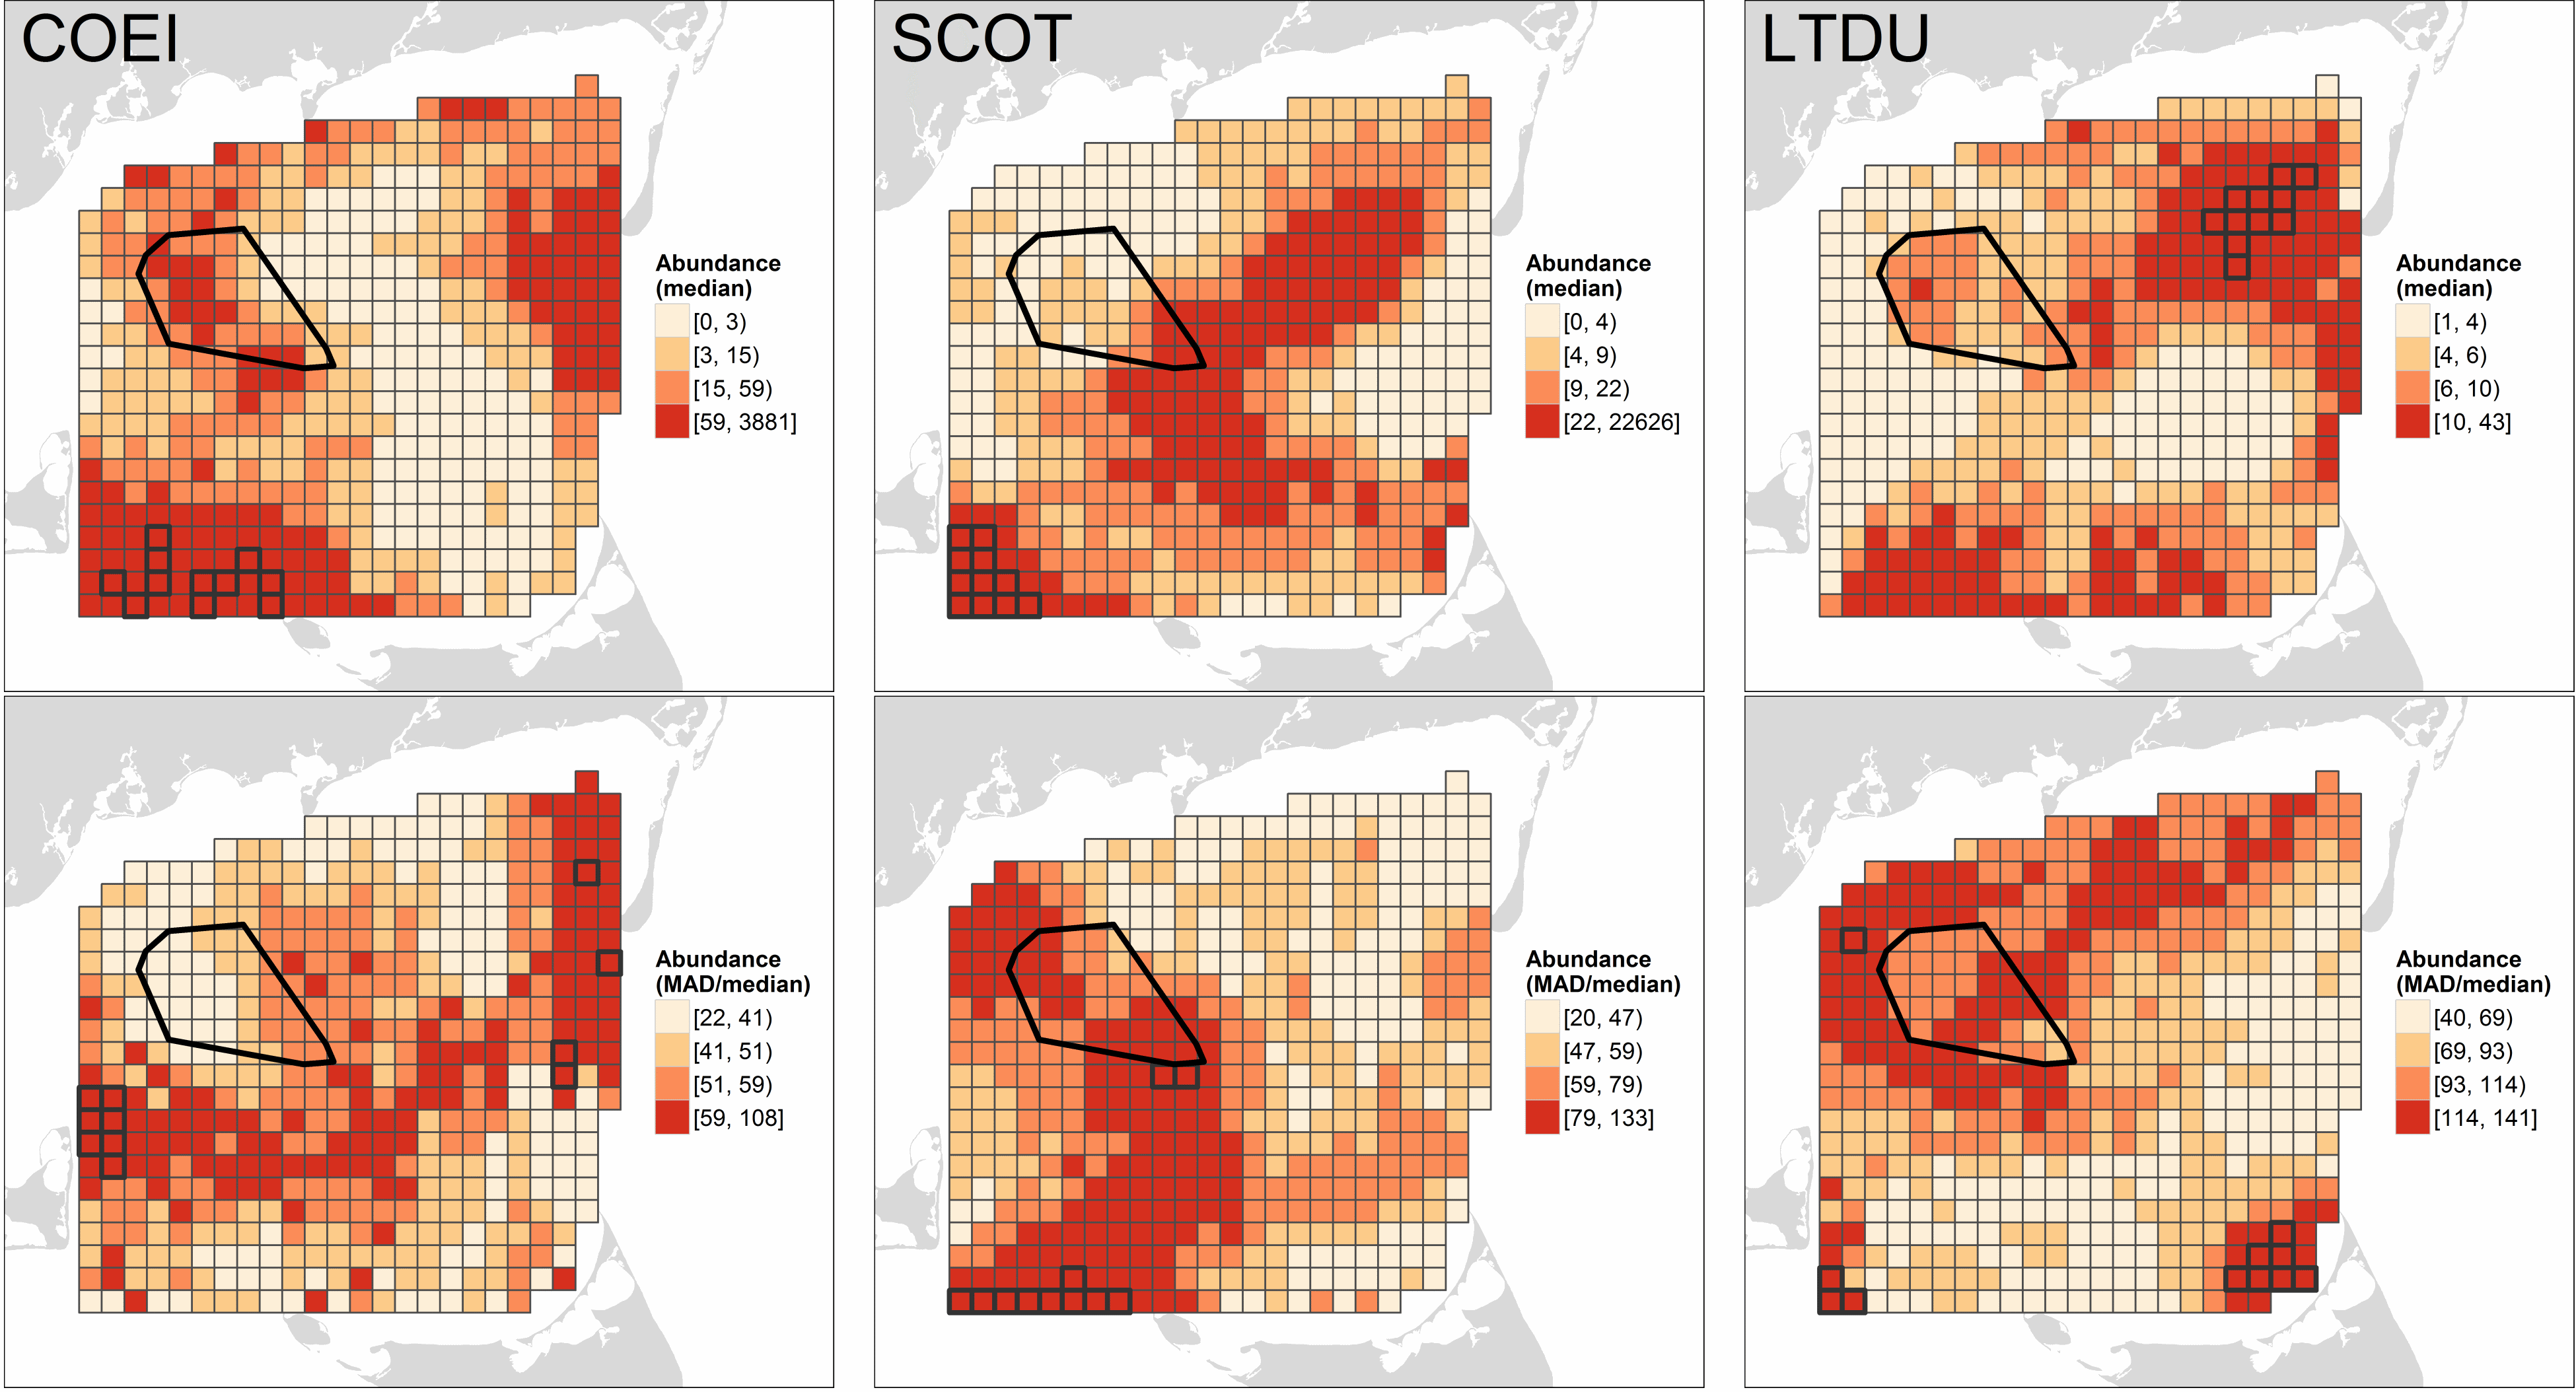
\includegraphics{./Figures/overall_abundance_maps_reduced.png}\\
\textbf{Figure 5}

\newpage

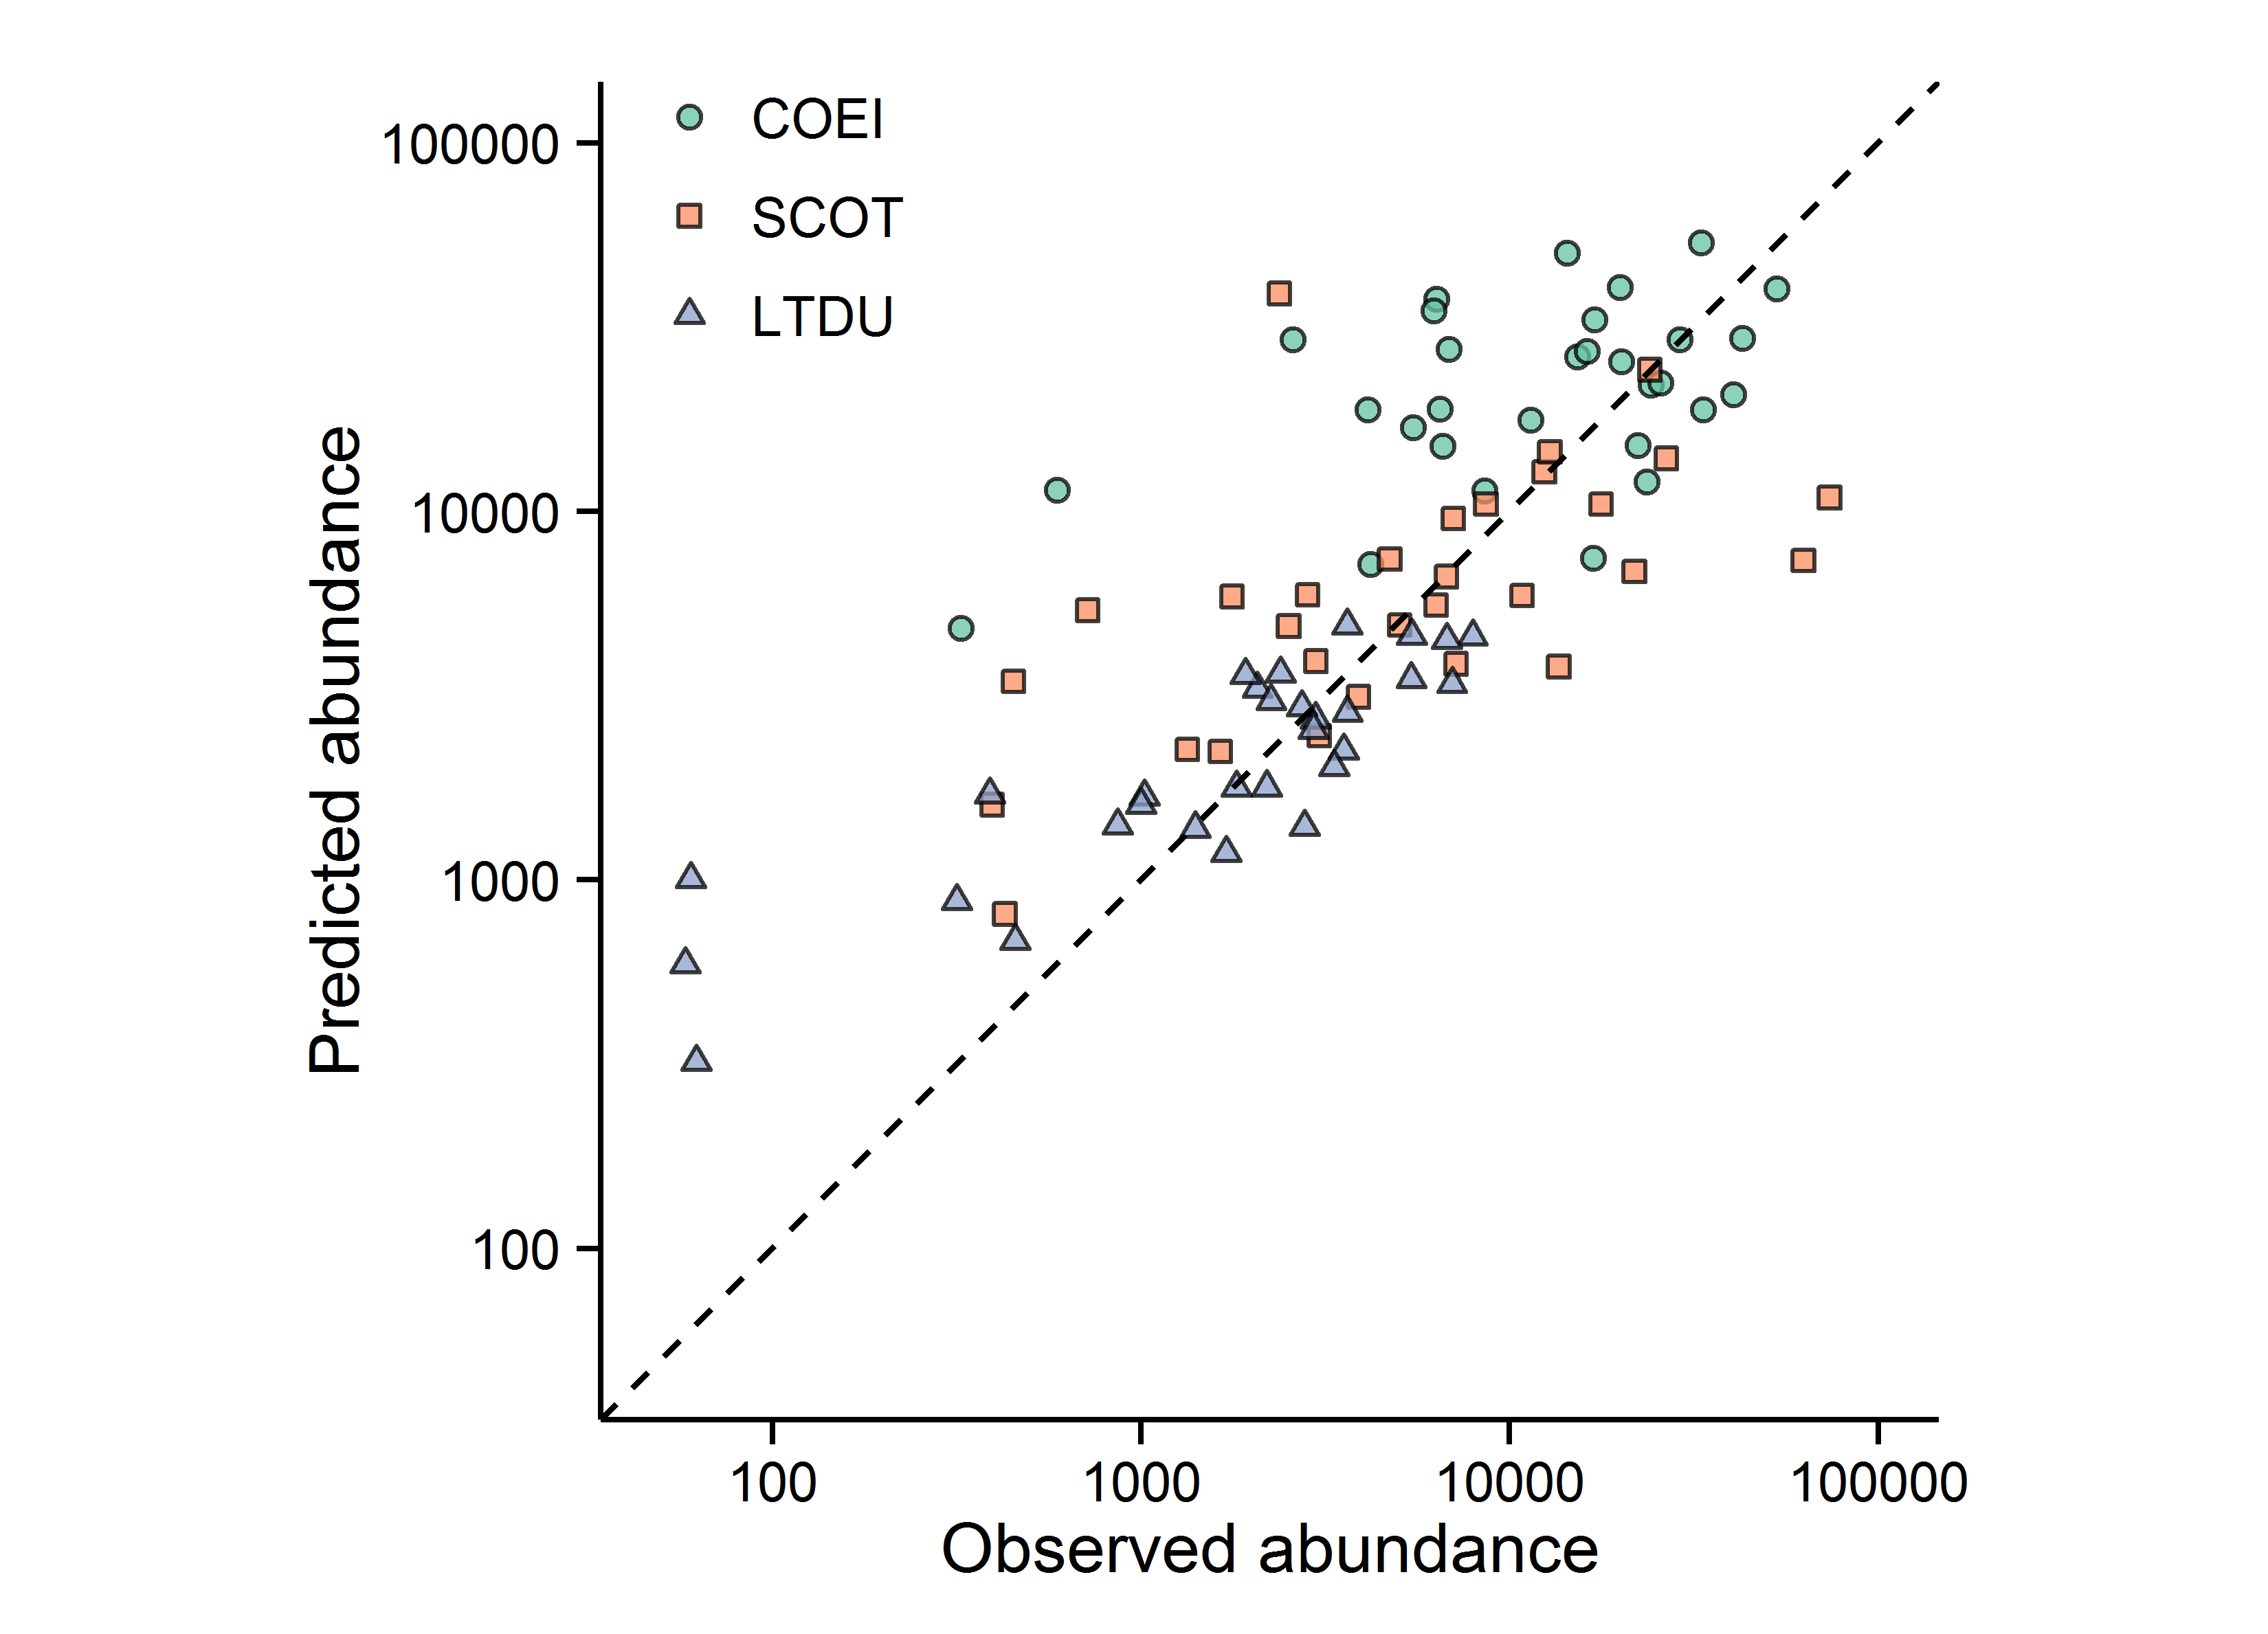
\includegraphics{./Figures/Predicted_abundance_observed_abundance.png}\\
\textbf{Figure 6}
